\documentclass[a4paper,10pt]{article}

\usepackage[english]{babel}
\usepackage{graphicx}
\usepackage[colorlinks, allcolors=black]{hyperref}
\usepackage{geometry}
\geometry{tmargin=3cm, bmargin=2.2cm, lmargin=2.2cm, rmargin=2cm}
\usepackage[colorinlistoftodos,prependcaption,textsize=small]{todonotes} %Used for the figure placeholder
\usepackage{minted}
\usepackage{color}
\usepackage{epstopdf}
\usepackage{lscape}
\usepackage{multirow}
\usepackage{subcaption}
\usepackage{amsmath}
\usepackage{lipsum}

\graphicspath{{../figures/}}

\begin{document}
\input{titlepage}
\tableofcontents

\section{Introduction}
In this report our algorithm for segmenting incisors is explained. Active shape models are used in combination with multi-resolution search to find the segmentation of the incisors. The algorithm is semi-automatic as bounding boxes have to be provided by the user.

\section{Active Shape Model}
In order to segment the incisors, an active shape model is built based on the provided training landmarks. A model is constructed for each individual incisor, resulting in eight models. This method is preferred over constructing one model for all incisors, because this would increase the variance of the landmarks.

To build this model, all the landmarks must first be aligned. This is achieved by Procrustes analysis. A principal component analysis is performed on the aligned segmentations in order to analyse the variations of the segmentations, and reduce the dimensionality and thus the complexity of the active shape model.
\subsection{Procrustes analysis}
The Procrustes analysis is done by taking the first segmentation sample and normalizing this sample. The other training examples are then optimally translated, scaled and then rotated to reduce the error between the corresponding landmark points. In the next iterations the reference sample is the mean of all the aligned segmentations. If the mean has converged, the process stops.

The optimal alignment is found by solving the weighted least squares problem, where the weights are based on the variance of the landmark points. High variance of a landmark means that the landmark is taken less into account in the error.

The result of the analysis is shown in figure \ref{fig:procrustes_single_tooth}.

\begin{figure}[htbp]
	\centering
	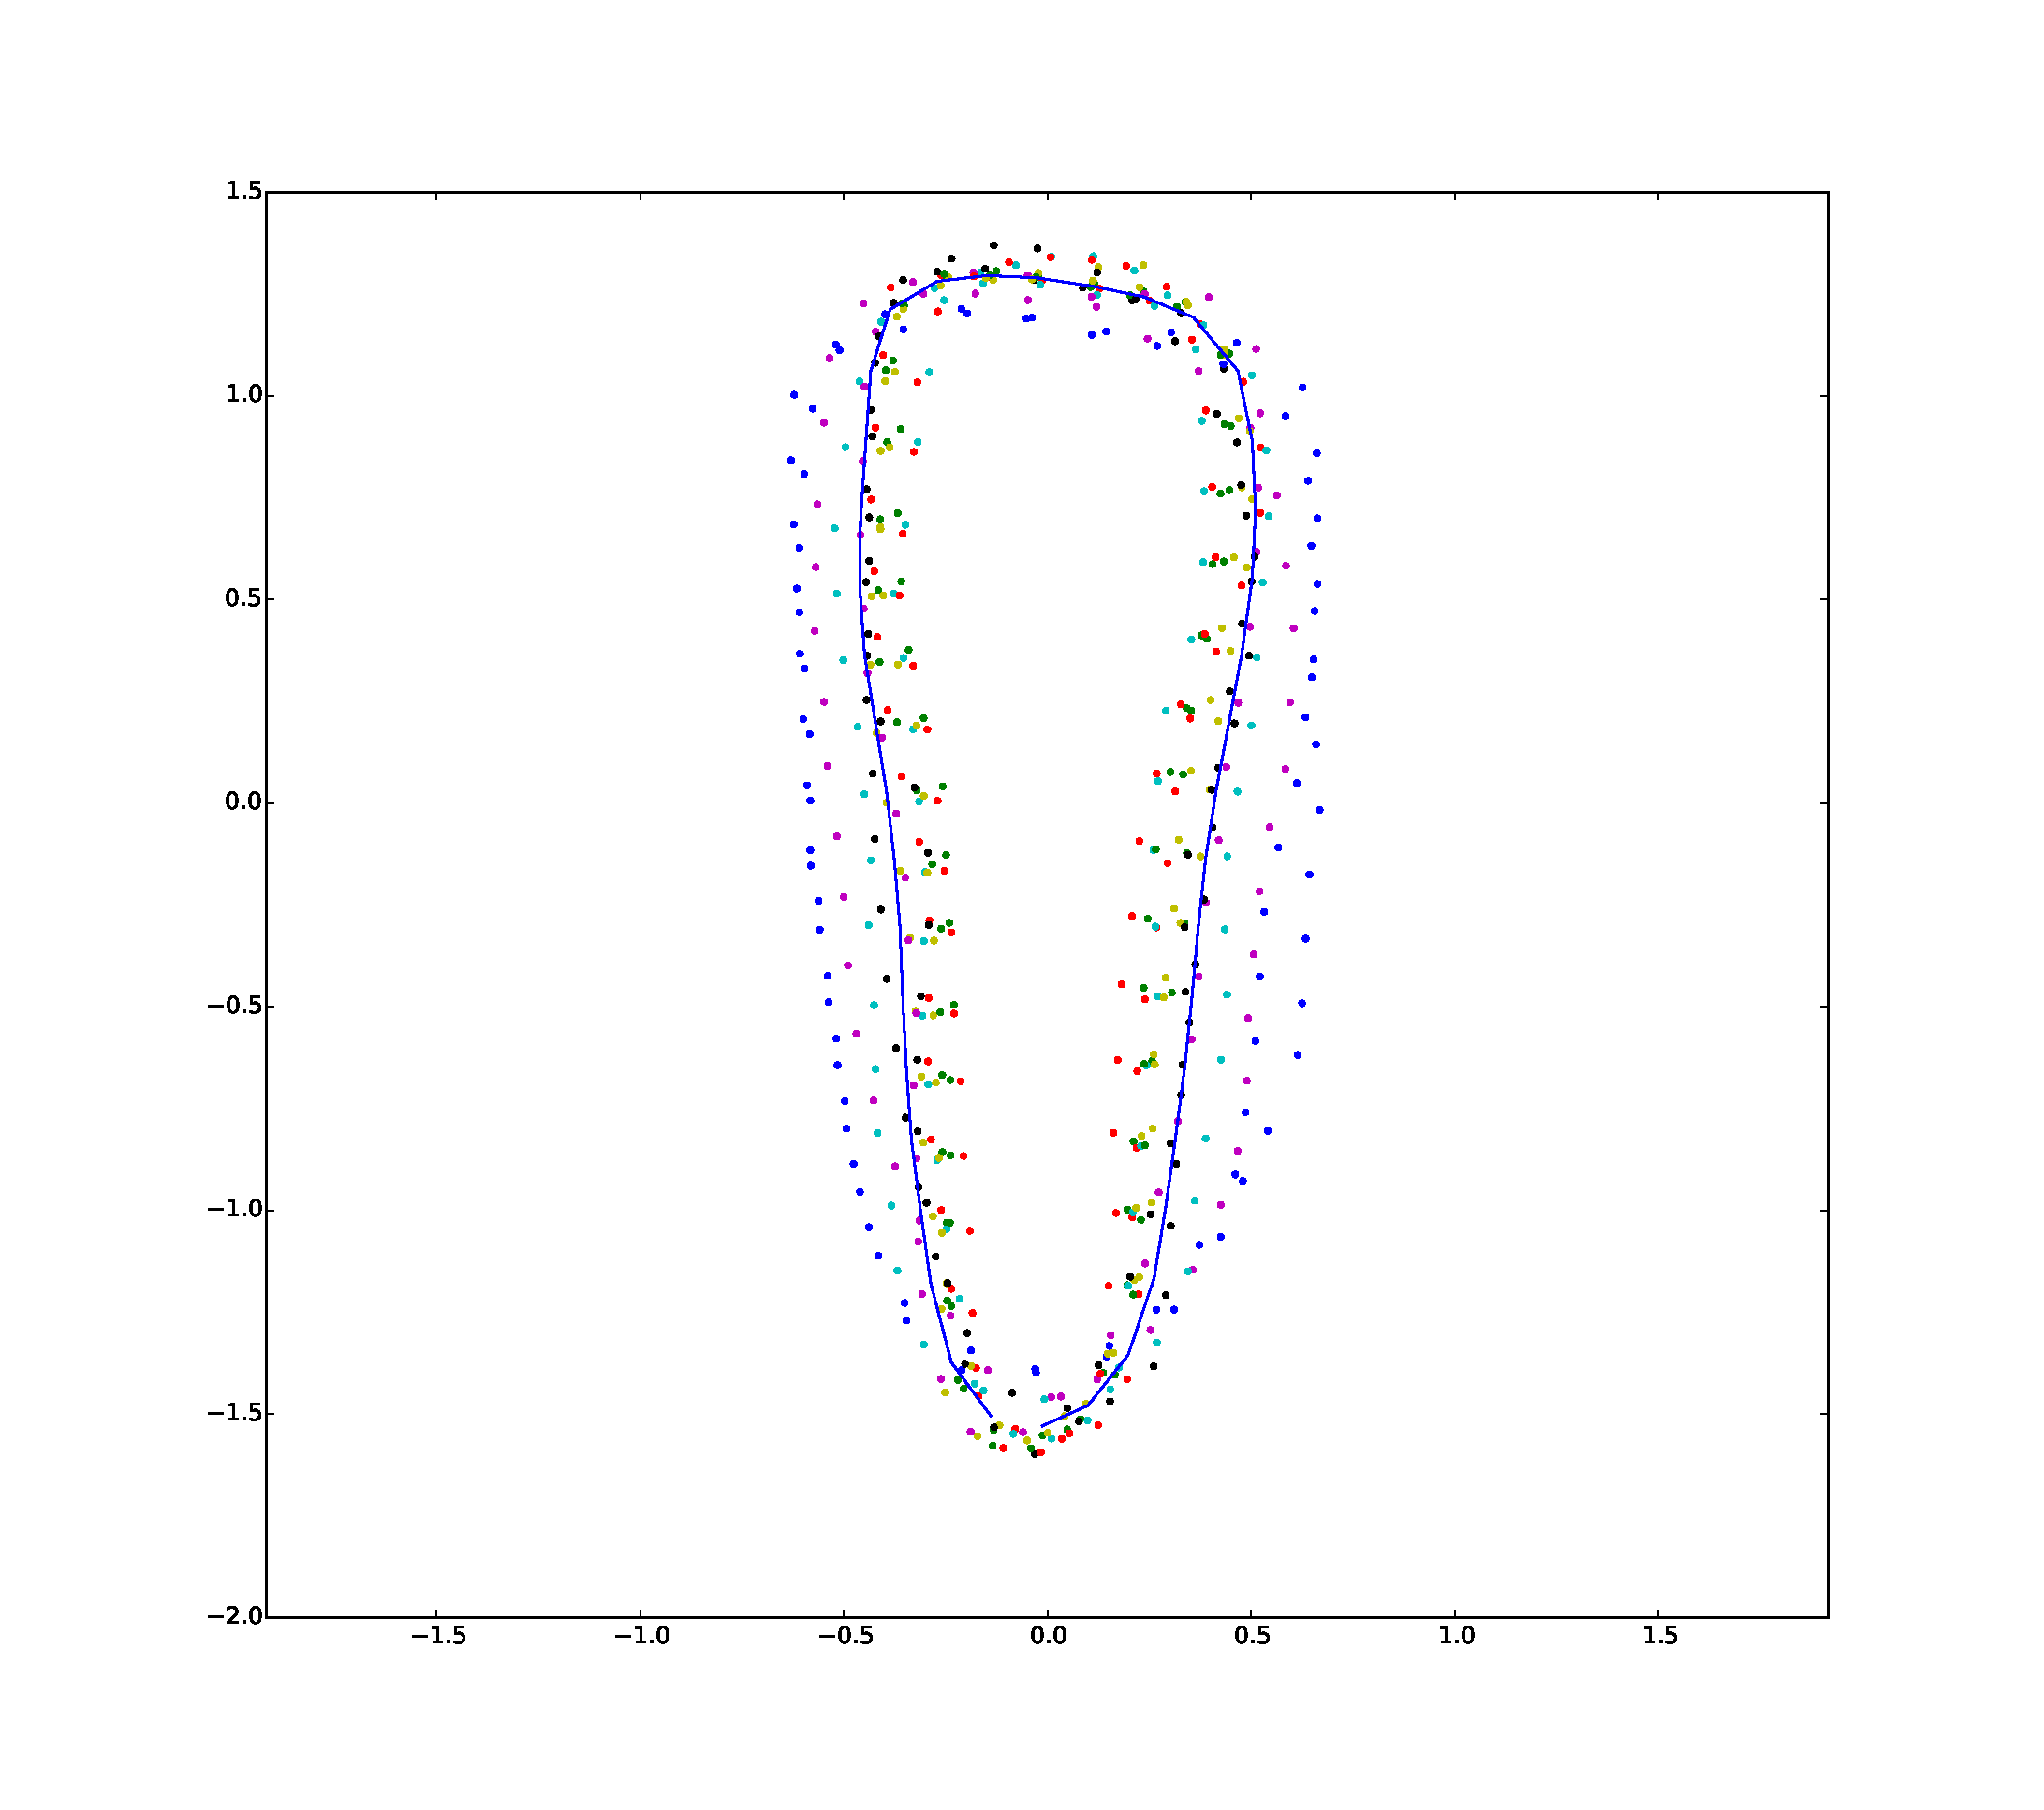
\includegraphics[width=0.9\textwidth, trim=0cm 2.5cm 0cm 3cm, clip]{procrustes_single_tooth}
	\caption{Alignment of training examples with the mean indicated for the third incisor}
	\label{fig:procrustes_single_tooth}
\end{figure}

\subsection{Principal component analysis}
The main objective of a principal component analysis is to reduce the dimensionality by representing the variables by principal components. These components are linear combinations of the variables. In order to keep as much information as possible, the components are chosen which explain the most variance. These components are the eigenvectors of the matrix containing the landmarks for the different images for one incisor. The eigenvectors corresponding to the highest eigenvalue explains the most of the variance. We chose to include the three first principal components for every incisor as these always explained between 80\% and 95\% of the variance. Notice that the 40 variables can be efficiently be reduced to only three components.

The principal components can be seen in figure \ref{fig:pca_components}. The information explained by the principal components can be interpreted from these figures. The first principal component explains the width of the tooth, the second component explains the skewness of the tooth and the third component explains the ratio between the width of the top and bottom of the tooth. These interpretations hold for every model.

\begin{figure}[htbp]
	\centering
	\begin{subfigure}{0.30\textwidth}
		\centering
		\includegraphics[width=\textwidth, trim=0cm 2.5cm 0cm 3cm, clip]{pca1_pos}
		\caption{Positive value for the first PCA component}
	\end{subfigure}
	~
	\begin{subfigure}{0.30\textwidth}
		\centering
		\includegraphics[width=\textwidth, trim=0cm 2.5cm 0cm 3cm, clip]{pca2_pos}
		\caption{Positive value for the second PCA component}
	\end{subfigure}
	~
	\begin{subfigure}{0.30\textwidth}
		\centering
		\includegraphics[width=\textwidth, trim=0cm 2.5cm 0cm 3cm, clip]{pca3_pos}
		\caption{Positive value for the third PCA component}
	\end{subfigure}
	\\
	\begin{subfigure}{0.30\textwidth}
		\centering
		\includegraphics[width=\textwidth, trim=0cm 2.5cm 0cm 3cm, clip]{pca1_neg}
		\caption{Negative value for the first PCA component}
	\end{subfigure}
	~
	\begin{subfigure}{0.30\textwidth}
		\centering
		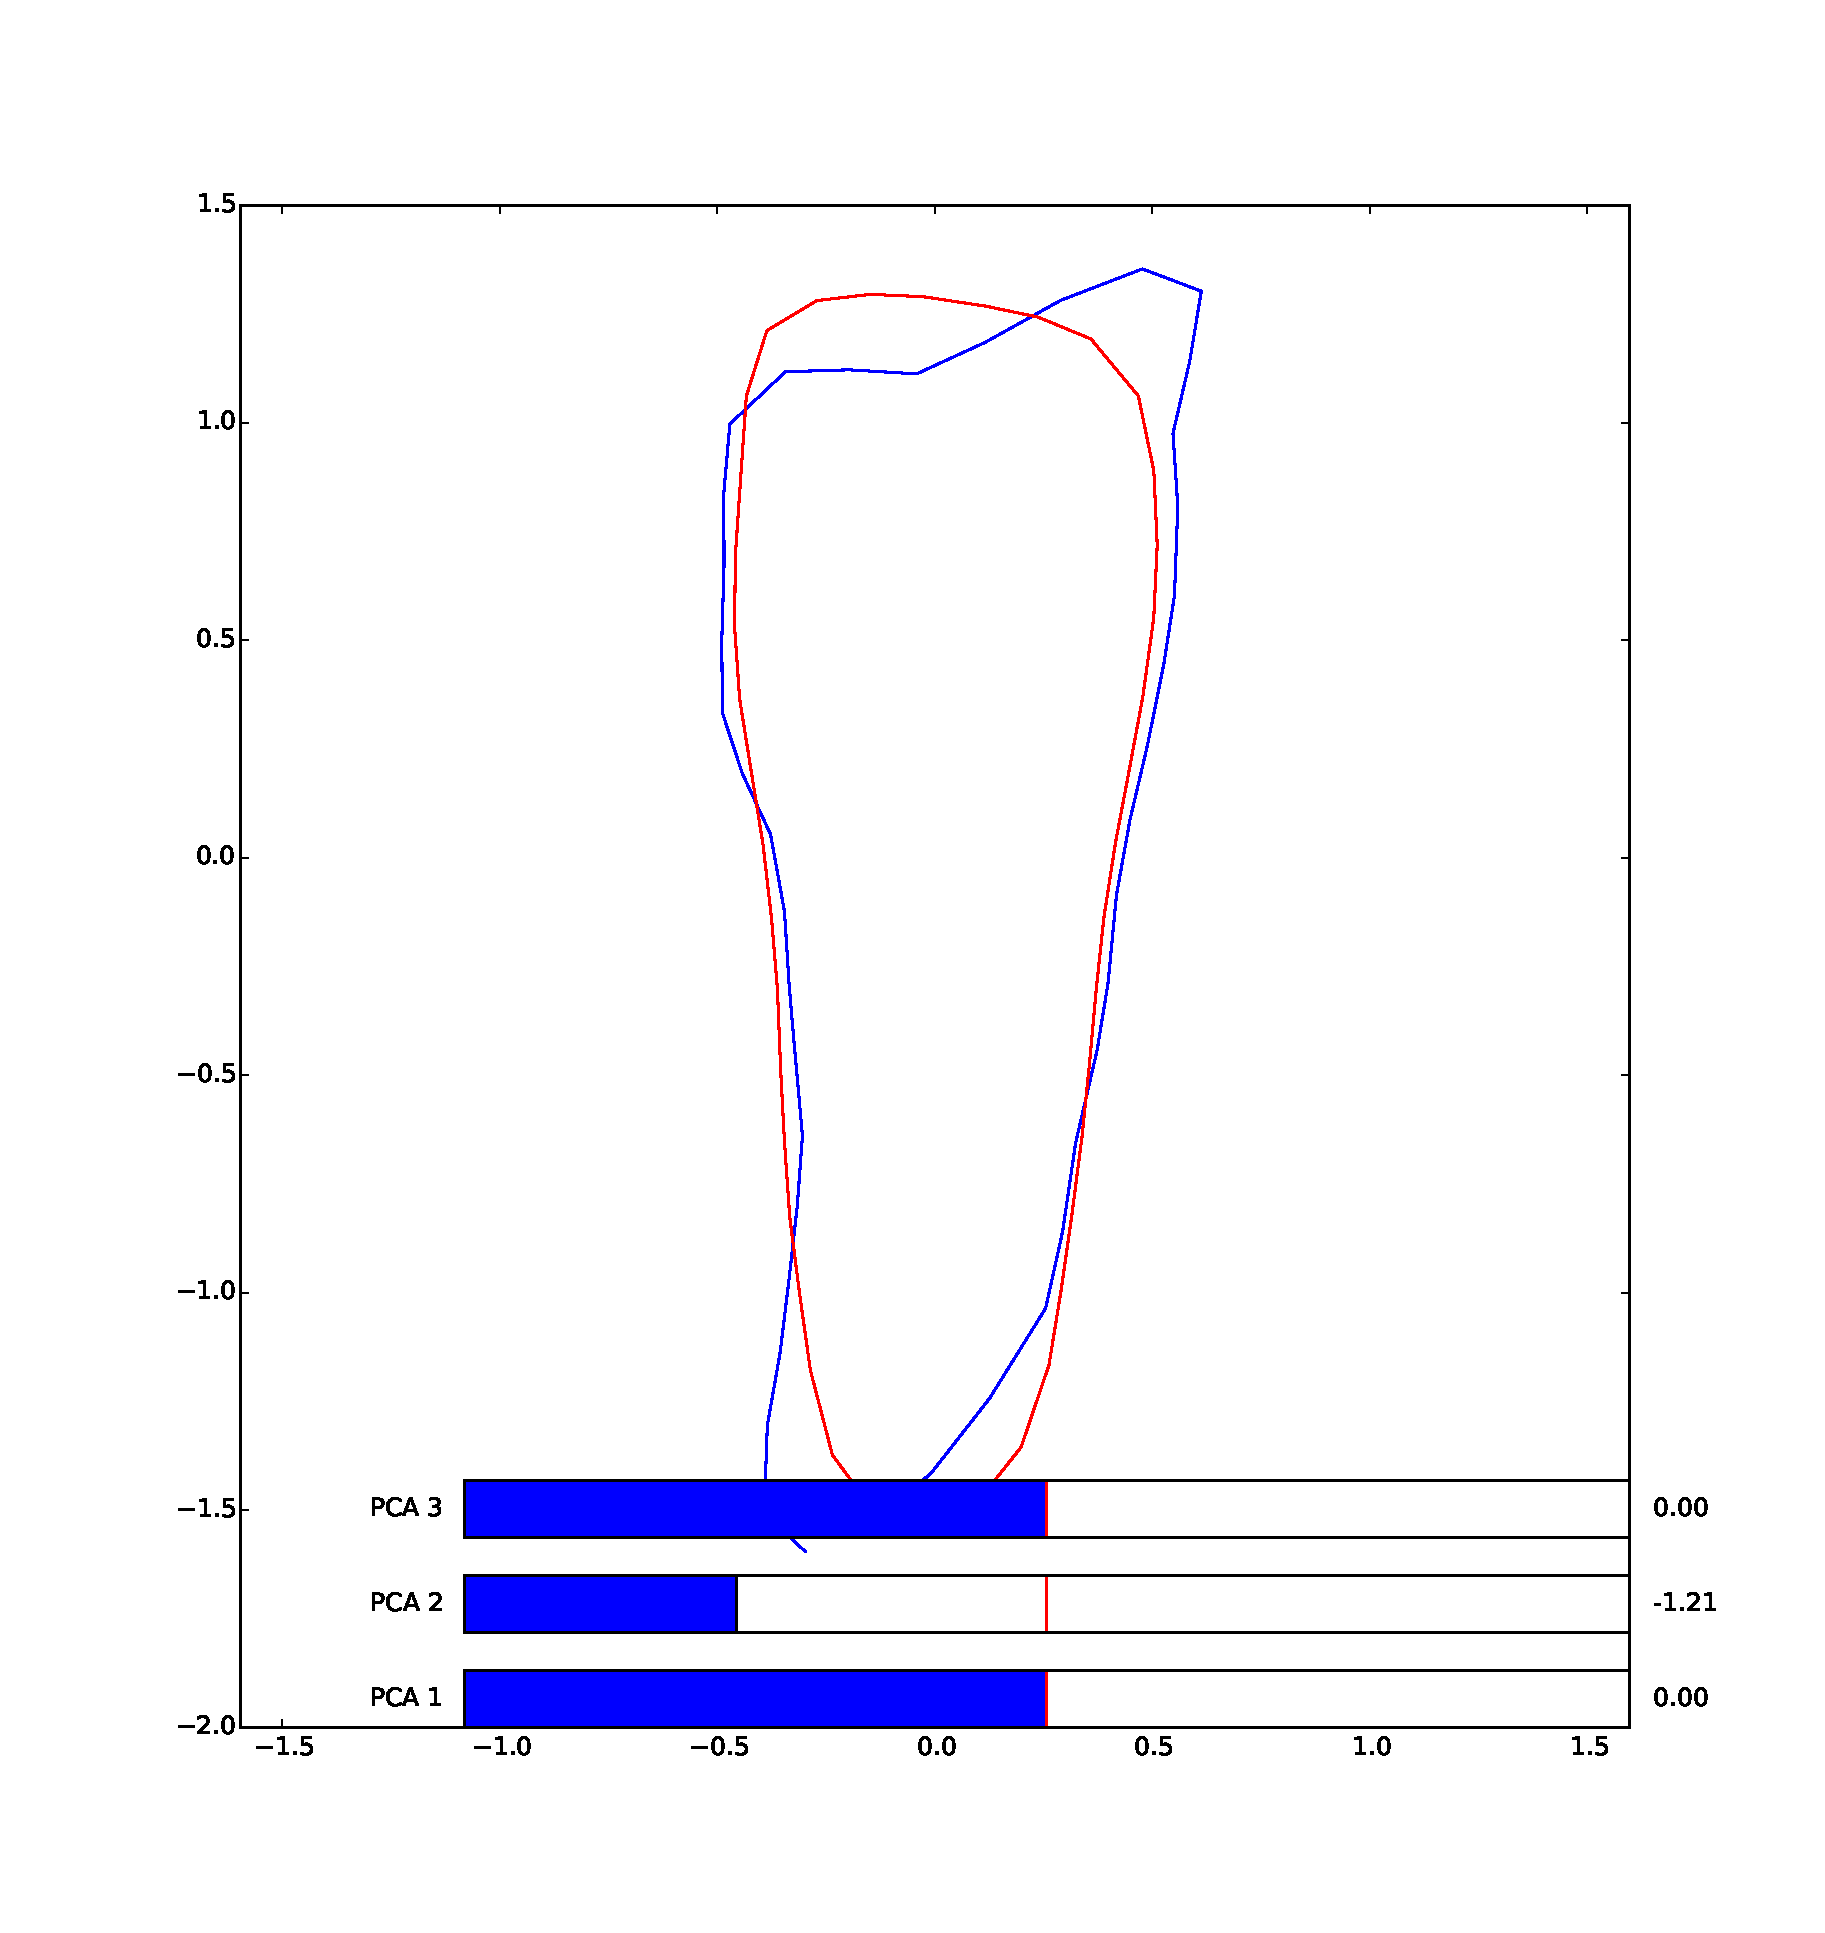
\includegraphics[width=\textwidth, trim=0cm 2.5cm 0cm 3cm, clip]{pca2_neg}
		\caption{Negative value for the second PCA component}
	\end{subfigure}
	~
	\begin{subfigure}{0.30\textwidth}
		\centering
		\includegraphics[width=\textwidth, trim=0cm 2.5cm 0cm 3cm, clip]{pca3_neg}
		\caption{Negative value for the third PCA component}
	\end{subfigure}
	\caption{PCA components; the mean model (red), adjusted model (blue)}
	\label{fig:pca_components}
\end{figure}

An approximation of the given segmentations by the model can be seen in figure \ref{fig:pca_tooth}. The exact landmarks of the tooth are plotted in green whereas the approximation is plotted in blue. This approximation is constructed by solving the following equation to find the parameter $b$:

\begin{equation*}
	x = \bar{x} + Pb
\end{equation*}

In this equation $\bar{x}$ is the mean model, $P$ is the projection matrix, containing the principal components and $x$ is the vector containing the exact landmarks of the tooth. $b$ is thus a weighting for each principal component, these values are shown in the bottom right in figure \ref{fig:pca_tooth}.


\begin{figure}[htbp]
	\centering
	\includegraphics[width=0.9\textwidth, trim=0cm 2.5cm 0cm 3cm, clip]{pca_tooth}
	\caption{Approximation (blue) of a tooth (green) for the third active shape model (red)}
	\label{fig:pca_tooth}
\end{figure}

\clearpage
\section{Segmentation of the dental radiographs}
The goal of segmentation of the dental radiographs is to find bounding boxes around different teeth. To achieve this the radiographs are first pre-processed. After this the gap valley of the denture is located. The next step would be to find the vertical gaps between the teeth. This last step wasn't accomplished. Manual bounding boxes were drawn to test further parts of the algorithm.
\subsection{Pre-processing}
The goal of this step is to highlight the dark parts in the gap valley to ease the searching for the gap valley. The two most important steps in this pre-processing are iterative and adaptive thresholding. Iterative thresholding tries to find an intensity threshold to distinguish teeth from other areas in the radiograph. As to not remove any parts of the teeth it is preferred to only remove the areas of which we are absolutely sure that they are not teeth. The result of this thresholding can be seen in figure \ref{fig:it_thresh}. Notice that the gap and some places between the teeth are partly black. The initial threshold value for iterative thresholding is based on the average intensity near edges. Canny is used to find these edges (see figure \ref{fig:dilate}). We assume that the most distinct edges correspond to teeth separations. The edges are dilated to find a better approximation for the initial thresholding value.

The last step is adaptive thresholding. This is shown in figure \ref{fig:ad_thresh}. Because the intensity of the radiograph varies in the image, a global thresholding does not perform good. Thresholding based on the intensity of the neighbourhood is accomplished by using adaptive thresholding. The results after iterative thresholding and adaptive thresholding can be seen in figure \ref{fig:result}. It can be seen that the gap valley is completely black.

\begin{figure}[htbp]
	\centering
	\begin{subfigure}{0.45\textwidth}
		\centering
		\includegraphics[width=\textwidth, trim=20cm 5cm 20cm 10cm, clip]{dilate}
		\caption{Blur + Canny + dilate}
		\label{fig:dilate}
	\end{subfigure}
	~
	\begin{subfigure}{0.45\textwidth}
		\centering
		\includegraphics[width=\textwidth, trim=20cm 5cm 20cm 10cm, clip]{it_thresh}
		\caption{Iterative thresholding}
		\label{fig:it_thresh}
	\end{subfigure}
	\\
	\begin{subfigure}{0.45\textwidth}
		\centering
		\includegraphics[width=\textwidth, trim=20cm 5cm 20cm 10cm, clip]{ad_thresh}
		\caption{Adaptive thresholding mask}
		\label{fig:ad_thresh}
	\end{subfigure}
	~
	\begin{subfigure}{0.45\textwidth}
		\centering
		\includegraphics[width=\textwidth, trim=20cm 5cm 20cm 10cm, clip]{result}
		\caption{Pre-processing result}
		\label{fig:result}
	\end{subfigure}
	\caption{Pre-processing steps (only a part of each image is shown)}
	\label{fig:pre_processing}
\end{figure}

\subsection{Gap valley detection}
Before searching for the gap valley a Gaussian filter is applied in the horizontal direction over the inverse of the pre-processed image. The idea behind this is that it is more important to find a good gap in the middle of the image, close to the incisors. In figure \ref{fig:paths} the effect of this filter can be seen.

To find the gap valley, intensity histograms are calculated at intervals over the width of the image. The intensities are the sum of the intensities lying in a horizontal range at each height. A plot of these intensities is shown in figure \ref{fig:fourier}. This histogram is then smoothed using a Fourier transformation. The maxima in this histogram represent points in the image through which the optimal path might pass. For each interval the four best points are kept as candidates. In the next step paths are generated between these points to find the optimal path. For each point an edge is added to the point with the lowest increase in intensity. The created paths are trimmed and then pruned based on their remaining length. The cost of the path is equal to the intensity of all points on this path in the original pre-processed image. The path with the lowest intensity corresponds to the gap valley. The maxima, remaining paths after pruning and the best path can be seen in figure \ref{fig:paths}.

\begin{figure}[htbp]
	\centering
	\includegraphics[width=0.9\textwidth, trim=0cm 2.5cm 0cm 3cm, clip]{fourier_intensity}
	\caption{Fourier transformation of intensity histogram for one vertical slice of the image \\(pixel index on x-axis, intensity on y-axis)}
	\label{fig:fourier}
\end{figure}

\begin{figure}[htbp]
	\centering
	\includegraphics[width=1\textwidth, trim=0cm 0cm 0cm 0cm, clip]{paths}
	\caption{The remaining horizontal paths after pruning (blue) and the horizontal path for the gap valley (yellow), with the line intensity on the pre-processed image}
	\label{fig:paths}
\end{figure}


\clearpage
\section{Fit the model to an image}
The fitting of the model can be divided in roughly four parts. First an initial guess is made where the mean model should be placed. As stated before, our algorithm does not automatically find a bounding box around the location of a tooth. The start of this algorithm thus requires a bounding box and a radiograph as input. The second step is the start of an iterative process, the pose and shape parameters of the current model are updated to approximate the points in the image. These points are searched in the image based on the intensity of the neighbourhood of the model landmarks. This neighbourhood was learned from the training set. To make the algorithm more robust against a bad initial guess this iterative process is repeated on different levels. A Gaussian pyramid was used to create the images for the different levels.
\subsection{Initial fit}
The initial placement of the mean model is based on the bounding box, given as input by the user. This is not ideal and thus has to be automatised. For a possible solution to this problem we refer to the previous section. The mean model is placed as large as possible in this bounding box. Depending whether the bounding box is placed above or below the horizontal gap, the mean model is placed close to the bottom or top edge of this bounding box respectively.

\subsection{Update pose and shape parameters to fit model to image landmarks}
The goal of this step is to find the $b$-vector that gives the best fit of the model to the current set of image points. This is done using an iterative process. The initial $b$-vector is zero, thus the initial model corresponds to the mean model. This model is transformed to align it as good as possible with the current set of image points using a Procrustes analysis. The new values for $b$ can then be calculated:
\begin{equation*}
	b = P^T(T^{-1}(Y)-\bar{x})
\end{equation*}
where $Y$ is the current set of image points and $T^{-1}$ is the inverse of the previous transformation. This process is repeated until the $b$-vector converges.

\subsection{Find landmarks on image based on neighbourhood near model points}
The goal of this step is to find `better' points near the current model points. To find these `better' points, a statistical model is constructed of the neighbourhood of the landmarks of the training examples. This intensity neighbourhood is the normal vector through the landmark point. It is assumed that this neighbourhood for a landmark is normally distributed over the training examples. Because of this the Mahalanobis distance between a provided neighbourhood and the model can be used to measure.

In figure \ref{fig:normal_vector} the normal vector of each landmark point is shown together with the point corresponding to the best match of the neighbourhood model. These best points are then used to find a new approximation model as explained in the second step.

The algorithm stops the iterative process if 90\% of the new best points lie sufficiently close to the current model or if the maximum amount of iterations is reached.

\begin{figure}[htbp]
	\centering
	\includegraphics[width=0.4\textwidth, trim=17cm 2cm 21cm 13.5cm, clip]{normal_vectors}
	\caption{Best point (black) on the normal (grey) for each current landmark (white)}
	\label{fig:normal_vector}
\end{figure}

\subsection{Multi-resolution fitting}
To improve the robustness of the searching of new landmark points in the image based on the neighbourhood, multi-resolution search is used. A Gaussian pyramid of three levels is constructed. As a consequence statistical models of the neighbourhoods on each level have to be constructed. The goal of this search method is to first search for the model on a high level. This allows the algorithm to find a rough estimate of the location of the incisor and search in lower levels for a more specific location of the model based on the model found in the higher level. Models after convergence of each level can be seen in figure \ref{fig:multi_res}.

\begin{figure}[htbp]
	\centering
	\begin{subfigure}{0.3\textwidth}
		\centering
		\includegraphics[width=1\textwidth, trim=280px 80px 240px 110px, clip]{level2}
		\caption{Level 2}
		\label{fig:level2}
	\end{subfigure}
	~
	\begin{subfigure}{0.3\textwidth}
		\centering
		\includegraphics[width=1\textwidth, trim=560px 160px 480px 220px, clip]{level1}
		\caption{Level 1}
		\label{fig:level1}
	\end{subfigure}
	~
	\begin{subfigure}{0.3\textwidth}
		\centering
		\includegraphics[width=1\textwidth, trim=1120px 320px 960px 440px, clip]{level0}
		\caption{Level 0}
		\label{fig:level0}
	\end{subfigure}
	\caption{Multi-resolution fitting: result for the three levels}
	\label{fig:multi_res}
\end{figure}

\clearpage
\section{Evaluation}
The evaluation of the gap valley detection was done manually on the fourteen original radiographs. In all these images the gap valley was found.

The evaluation of the segmentation of the incisor was done using leave-one-out cross validation for each incisor model. The average Euclidean distance in pixels between the found model and the given test example is used to evaluate the models. This leads to the following result for the eight models:


\begin{table}[h]
	\centering
	\begin{tabular}{l|llllllll}
		{\bf Incisor model}          & 0     & 1     & 2     & 3     & 4     & 5     & 6     & 7      \\ \hline
		{\bf Average pixel distance} & 36.81 & 27.73 & 25.80 & 34.58 & 18.17 & 16.80 & 19.05 & 19.01
	\end{tabular}
	\caption{Average pixel distances for different models}
\end{table}

We can conclude that the incisors of the bottom jaw are better fitted than the incisors of the upper jaw. This could be due to difference in variance of the upper and lower incisors.

In figure \ref{fig:evaluation} the fitted models are shown in black while the white points are the provided landmarks. In this figure it can also be seen that the fitted models sometimes (incisor 0 and 6) tend to go the the middle of a tooth if the tooth has a darker region. The reason for this is that the neighbourhood of this darker region is similar to an edge of a tooth.

\begin{figure}[htbp]
	\centering
	\includegraphics[width=1\textwidth, trim=400px 0 400px 200px, clip]{evaluation}
	\caption{Evaluation of the algorithm: given landmarks (white) versus the fitted model (black)}
	\label{fig:evaluation}
\end{figure}
\newpage
\bibliographystyle{plain}
\nocite{*}
\bibliography{bibtex}

\end{document}
